\section{\K 阻抗的串联与并联}
\begin{figure}[htbp]
	\centering
	\begin{minipage}[b]{0.45\textwidth}
        \centering
        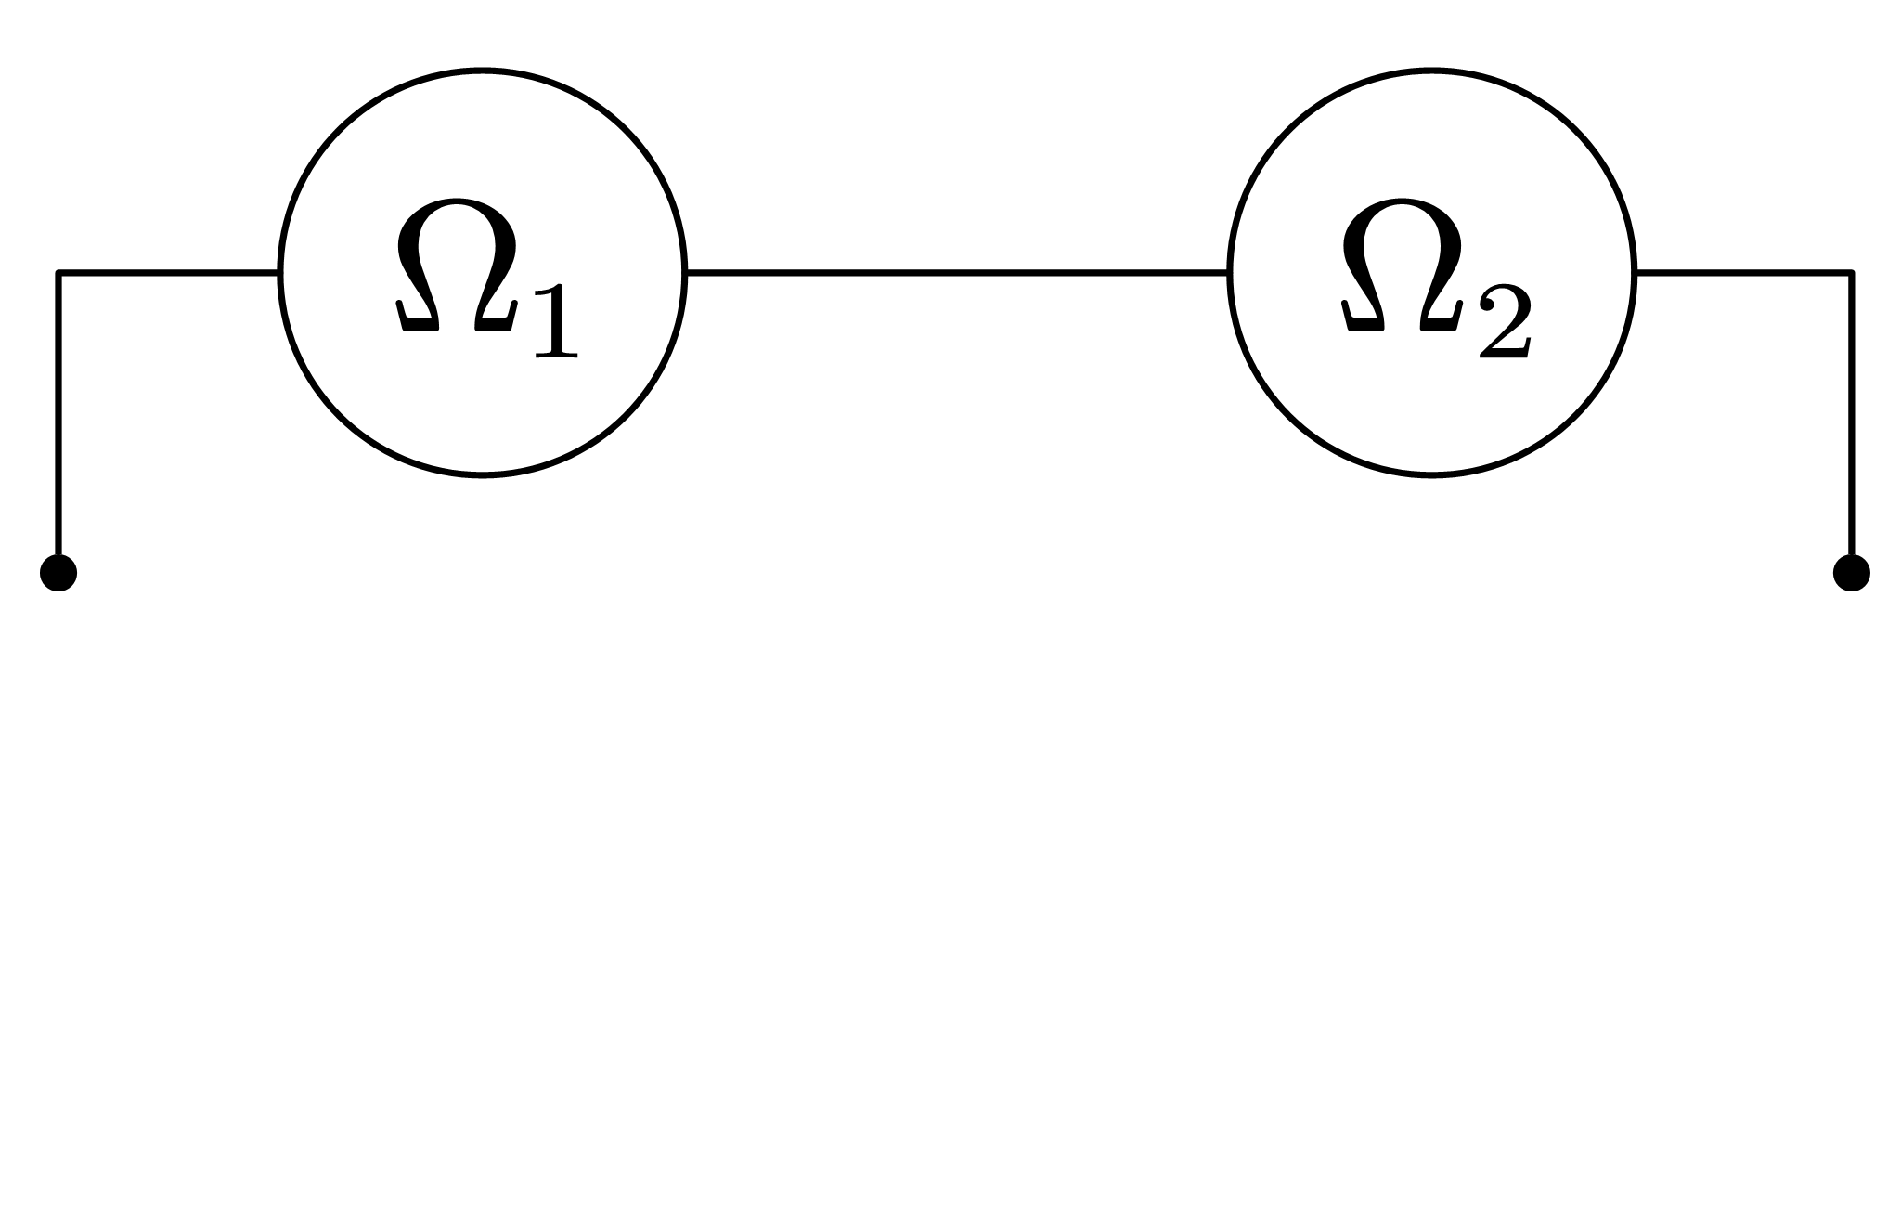
\includegraphics[width=0.65\textwidth]{串联阻抗.pdf}
        \caption{串联阻抗}
        \label{fig:串联阻抗}
    \end{minipage}
    \begin{minipage}[b]{0.45\textwidth}
        \centering
        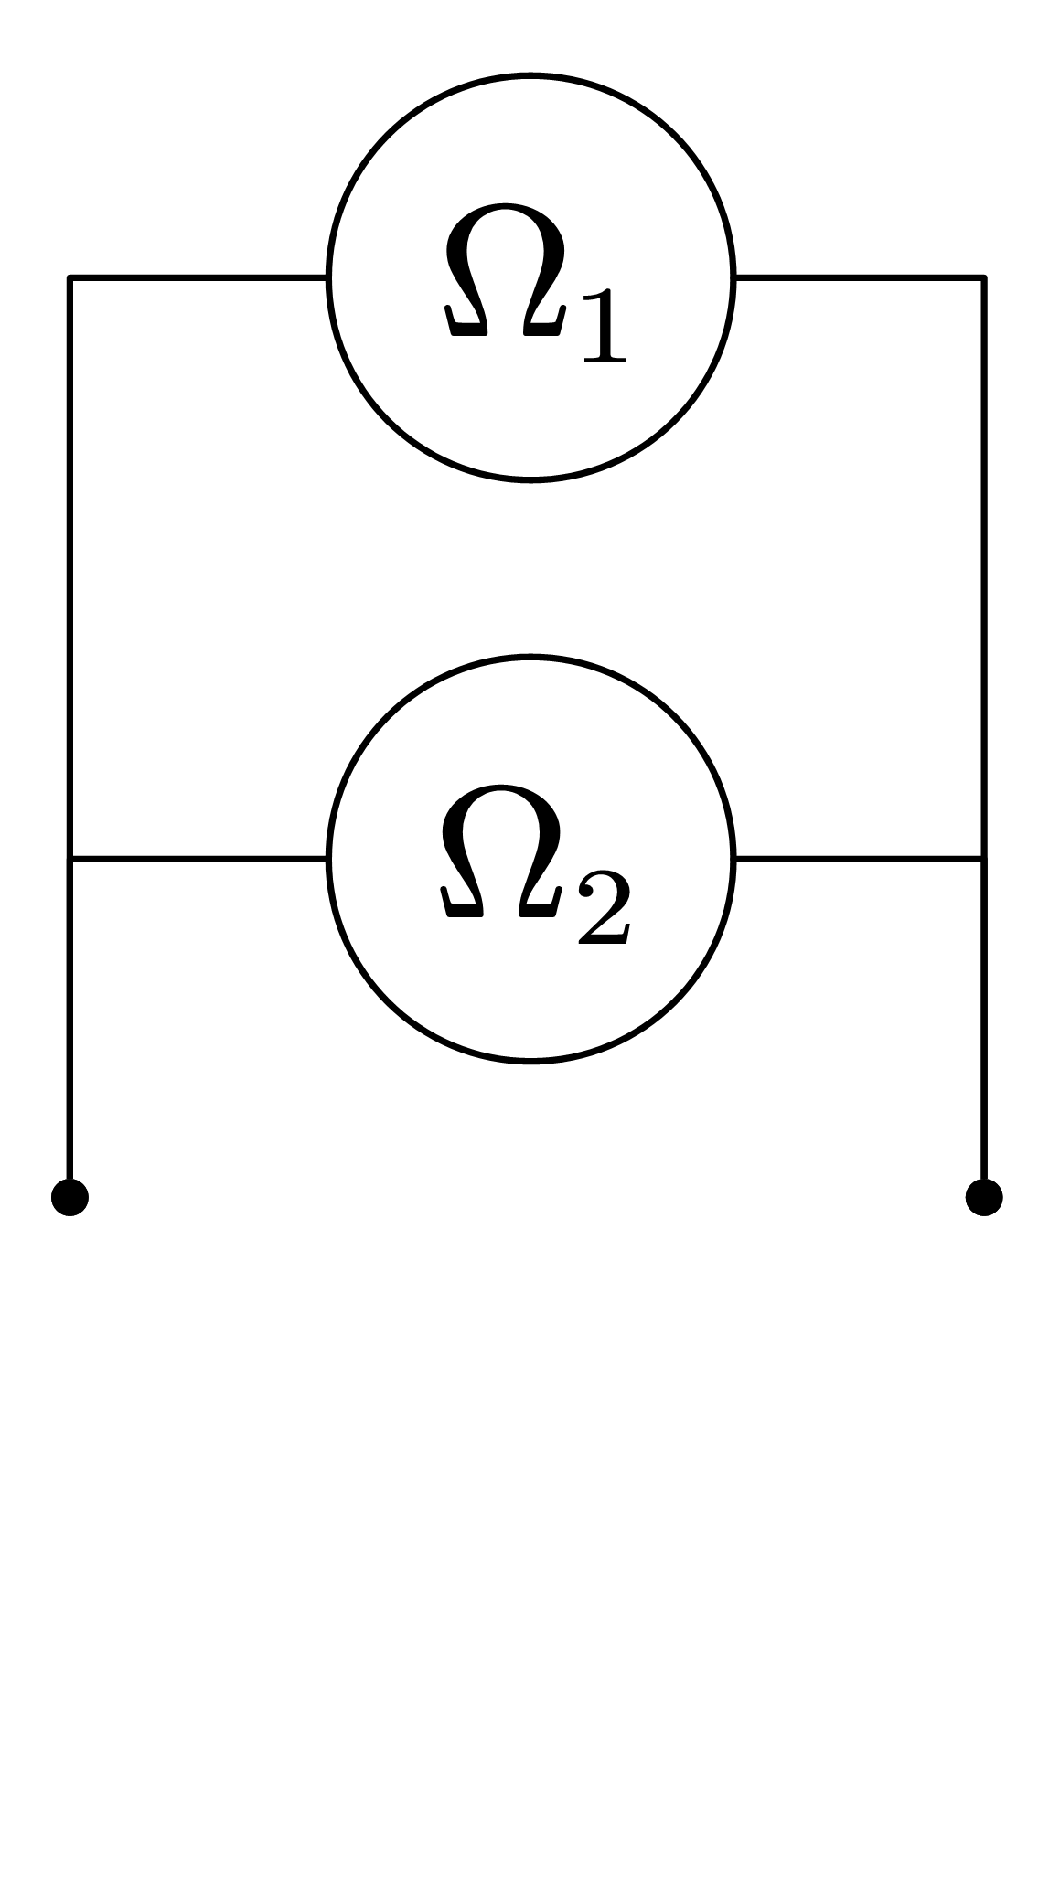
\includegraphics[width=0.65\textwidth]{并联阻抗.pdf}
        \caption{并联阻抗}
        \label{fig:并联阻抗}
    \end{minipage}
\end{figure}
\Par 如图\ref{fig:串联阻抗}所示,现有两个阻抗串联,我们根据基尔霍夫电压定律可以得到
\begin{equation}
    \dot{U}=\dot{U}_1+\dot{U}_2=Z_1\dot{I}+Z_2\dot{I}=\left( Z_1+Z_2 \right) \dot{I}
\end{equation}
由此,我们可以得到它的等效阻抗
\begin{equation}
    Z=Z_1+Z_2
\end{equation}
这就是\hl{阻抗的串联定律}.需要注意的是,一般来说,等效阻抗的阻抗模和阻抗角都不满足直接求代数和,只有等效阻抗等于串联阻抗的代数和.

\Par 同理,如图\ref{fig:并联阻抗}所示,我们用基尔霍夫电流定律可以得到
\begin{equation}
    \dot{I}=\dot{I}_1+\dot{I}_2=\frac{\dot{U}}{Z_1}+\frac{\dot{U}}{Z_2}=\dot{U}\left( \frac{1}{Z_1}+\frac{1}{Z_2} \right) 
\end{equation}
那么它的等效阻抗就为
\begin{equation}
    \frac{1}{Z}=\frac{1}{Z_1}+\frac{1}{Z_2}
\end{equation}
这就是\hl{阻抗的并联定律}.
